\documentclass[11pt]{article}
\usepackage[paperwidth=8.5in, paperheight=11in]{geometry}
\usepackage{algorithm}
\usepackage{algorithmicx}
\usepackage[noend]{algpseudocode}

\usepackage{../tjimo}

\newcommand{\sevenpoints}{Time limit: 45 minutes.}
\newcommand{\righthead}{\fdbox{Round}{Power}}

\usepackage{tikz}
\usepackage{amsmath}
\usepackage{amsthm}
\usepackage{amssymb}
\usepackage{enumerate}
\usepackage{gensymb}

\begin{document}

Unlike the other rounds, just getting the answer right is not enough on the Power Round. Make sure you explain your answer and use words
to describe how you arrived at your answer. In the words of middle school math teachers across the nation -- no work, no credit!

This Power Round is divided into two sections. In the first section, the shoelace theorem is defined and discussed.
In the second section, which is divided into multiple subsections, we will prove shoelace theorem for triangles. Note that you can use results from previous problems to prove a problem (that is, you can use Problem 1 to prove Problem 3, but not vice versa). 

\section{Introduction}

The shoelace theorem can be used to calculate the area of polygons, given the Cartesian coordinates of the vertices. 

\begin{theorem} (The Shoelace Theorem) Suppose the polygon $P$ has vertices $(a_1, b_1)$, $(a_2, b_2)$, ... , $(a_n, b_n)$, listed in counterclockwise order. Then the area of $P$ is

\[\dfrac{1}{2} |(a_1b_2 + a_2b_3 + \cdots + a_nb_1) - (b_1a_2 + b_2a_3 + \cdots + b_na_1)|\]
\end{theorem}

The Shoelace Theorem gets its name because if one lists the coordinates in a column, 
\begin{align*} 
(a_1 &, b_1) \\ 
(a_2 &, b_2) \\ 
& \vdots \\ 
(a_n &, b_n) \\ 
(a_1 &, b_1) \\ 
\end{align*} 
and marks the pairs of coordinates to be multiplied, the resulting image looks like laced-up shoes.


\begin{problem}[2 points total]
Find, with proof, the area of the nonagon below:
\begin{center}
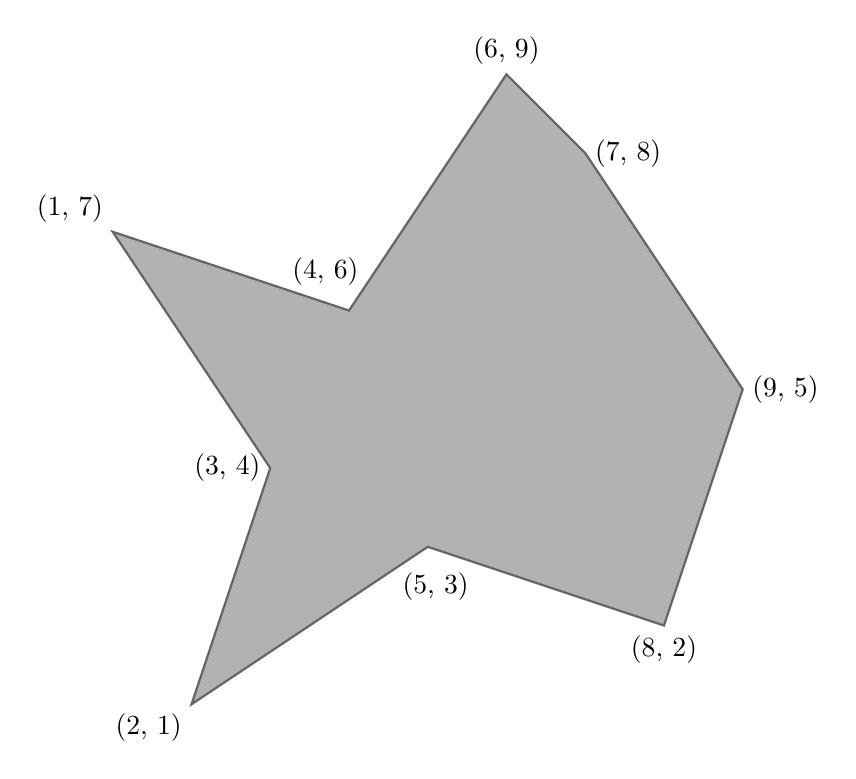
\begin{tikzpicture}
\filldraw[color = black!60, fill = black!30, thick] (6, 9) -- (4, 6) -- (1, 7) -- (3, 4) -- (2, 1) -- (5, 3) -- (8, 2) -- (9, 5) -- (7, 8) -- cycle;
\node at (6, 9) [above] {(6, 9)};
\node at (3.7, 6.2) [above] {(4, 6)};
\node at (1, 7) [above left] {(1, 7)};
\node at (3, 4) [left] {(3, 4)};
\node at (2, 1) [below left] {(2, 1)};
\node at (5.1, 2.8) [below] {(5, 3)};
\node at (8, 2) [below] {(8, 2)};
\node at (9, 5) [right] {(9, 5)};
\node at (7, 8) [right] {(7, 8)};
\end{tikzpicture}
\end{center}
\end{problem}

\begin{answer} 41 \end{answer}
\begin{solution} Plugging the vertices into the shoelace theorem, we see that the area is 
\[\dfrac{1}{2} |(6)(6) + (4)(7) + (1)(4) + (3)(1) + (2)(3) + (5)(2) + (8)(5) + (9)(8) + (7)(9)\]
\[-((6)(8) + (4)(9) + (1)(6) + (3)(7) + (2)(4) + (5)(1) + (8)(3) + (9)(2) + (7)(2))|\]
\[=\frac{1}{2}(262-180)=\boxed{41}\]
\end{solution}

%\begin{problem} \normalfont Prove that the shoelace theorem works for a triangle with a vertex at $(0, 0)$ and a base on the x-axis.


%\begin{problem} \normalfont Prove that the shoelace theorem works for squares with one vertex on the x-axis and one vertex on the y-axis.

\section{Areas of Triangles}

We will begin proving shoelace theorem for just triangles.

\subsection{Vertex at the Origin}
\normalfont Let the three vertices of triangle $ABC$ lie at $(0, 0), (x_1, y_1),$  and $(x_2, y_2)$.

\begin{problem} \normalfont Prove that the shoelace theorem applies to the following cases for $x_1, y_1, x_2, y_2 \geq 0$: (Hint: Draw a box around the triangle and subtract out unnecessary areas)
\begin{enumerate}[label=(a)]
\item $x_1 \leq x_2$ and $y_1 \geq y_2$
\item $x_1 < x_2$ and $y_1 < y_2$
\end{enumerate}
\end{problem}

\begin{solution} 
The area is $x_2y_1 - (\frac{1}{2}x_1y_1+\frac{1}{2}x_2y_2+\frac{1}{2}(x_2-x_1)(y_1-y_2))$.
Expanding and cancelling gives $\frac{1}{2}(x_2y_1-x_1y_2)$. Note that this is the same result as when we use shoelace.

Note that there are two cases. 
\newline \textbf{Case 1:} $(x_2, y_2)$ is above the diagonal
The area is $x_1y_1 - (\frac{1}{2}(x_1-x_2)(y_1-y_2)+\frac{1}{2}x_2y_2+(x_2)(y_1-y_2)+\frac{1}{2}x_1y_1)$.
Expanding and cancelling gives $\frac{1}{2}(x_2y_1-x_1y_2)$. 
\newline \textbf{Case 2:} $(x_2, y_2)$ is below the diagonal
The area is $x_1y_1 - (\frac{1}{2}(x_1-x_2)(y_1-y_2)+\frac{1}{2}x_2y_2+(y_2)(x_1-x_2)+\frac{1}{2}x_1y_1)$.
Expanding and cancelling gives $\frac{1}{2}(x_2y_1-x_1y_2)$. 

Note that this is the same result as when we use shoelace.
\end{solution}


\begin{problem} \normalfont Prove that the shoelace theorem applies when $(x_1, y_1)$ lies in the first quadrant and $(-x_2, y_2)$ lies in the second quadrant. \end{problem}

\begin{solution}

\end{solution}

\begin{problem} \normalfont Prove that the shoelace theorem applies when $(x_1, y_1)$ lies in the first quadrant and $(-x_2, -y_2)$ lies in the third quadrant. \end{problem}

\begin{problem} \normalfont Prove that the shoelace theorem is consistent when a triangle is rotated by $90\degree$ clockwise or counterclockwise about the origin. Assume that one vertex remains at the origin. \end{problem}

\begin{problem} \normalfont Prove that shoelace theorem applies given any triangle with a vertex at the origin. \end{problem}

\subsection{General Triangles}
\begin{problem} \normalfont Prove that the shoelace theorem is consistent with translation, or in other words, the triangle with vertices $(x_1, y_1), (x_2, y_2), (x_3, y_3)$ has the same area as the triangle with vertices $(x_1 - a, y_1 - b), (x_2 - a, y_2 - b ), (x_3 - a, y_3 - b)$. \end{problem}

\begin{problem} \normalfont Prove that the shoelace theorem applies for all triangles. \end{problem}

\subsection{Clockwise or Counterclockwise?}
Note that for the 6 ways of ordering the vertices of the triangle, each ordering will traverse the vertices in either a clockwise or a counterclockwise direction. 
\newline \noindent Let the three vertices of triangle $ABC$ lie at $(x_1, y_1), (x_2, y_2),$  and $(x_3, y_3)$, in counterclockwise direction starting at $(x_1, y_1)$. 
Let $S_1$ be the sum $x_1 \bullet y_2 + x_2 \bullet y_3 + x_3 \bullet y_1$, and $S_2$ be the sum $x_2 \bullet y_1 + x_3 \bullet y_2 + x_1 \bullet y_3$.

\begin{problem} \normalfont Prove that
\[\left|\begin{array}{c c} x_1 &  y_1 \\ x_2  & y_2 \\ x_3  & y_3 \\ x_1 & y_1 \\ \end{array}\right| = 
\left|\begin{array}{c c} x_2  & y_2 \\ x_3  & y_3 \\ x_1 &  y_1 \\ x_2 & y_2 \\ \end{array}\right| = 
\left|\begin{array}{c c} x_3  & y_3 \\ x_1 &  y_1 \\ x_2  & y_2 \\ x_3 & y_3 \\ \end{array}\right| = 
-\left|\begin{array}{c c}x_1 &  y_1 \\ x_3  & y_3 \\ x_2  & y_2 \\ x_1 & y_1 \\ \end{array}\right| = 
-\left|\begin{array}{c c} x_2  & y_2 \\ x_1  & y_1 \\ x_3 &  y_3 \\ x_2 & y_2 \\ \end{array}\right| = 
-\left|\begin{array}{c c} x_3  & y_3 \\ x_2 &  y_2 \\ x_1  & y_1 \\ x_3 & y_3 \\ \end{array}\right|\]

\end{document}
